u\subsubsubsubsection{Bikepath Factory}
\begin{figure}[h]
\centering
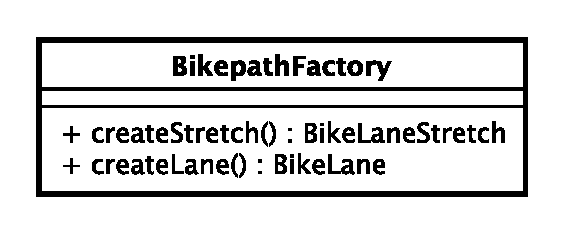
\includegraphics[scale=0.6,keepaspectratio]{images/solution/bikepath_factory.eps}
\caption{\pReactiveFactory::factory::BikepathFactory}
\label{fig:sd-app-bikepath-factory}
\end{figure}
\FloatBarrier
\begin{itemize}
  \item \textbf{\descr} \\
It represents a factory which creates bikepath components.
  \item \textbf{\ops} \\
  \begin{itemize} 
    \item[+] \texttt{createStretch() : BikeLaneStretch} \\
Creates a new bike lane stretch component.
    \item[+] \texttt{createLane() : BikeLane} \\
Creates a new bike lane component.
  \end{itemize}
\end{itemize}
